\subsection{Feasibility and Success Criteria }
The success of this project depends on meeting the performance metrics and thereby achieving the goals mentioned in the mission statement. Table \ref{Tab:msc} indicates how those metrics will be for measured and whether the proposal holds true  during testing phase.

Based on feasibility Table on the right and the project analysis provided shows the importance of orbital flight for weather satellites. 
Highlighting  the severity of the consequences associated with hurricane activity, not only is orbital flight beneficial but crucial to the likes of NASA in order to  mitigate & alert public safety from a catastrophic weather. Project Hurrisat proves it is indeed possible to tackle down hurricanes effectively and perhaps avoiding them in an efficient manner for years to come.  \\
\begin{table}[h]
\caption{Mission Success Criteria}
\begin{tabular}{lll}
\rowcolor[HTML]{C0C0C0} 
Objective &
  Effective Measure &
  Control Method \\ \hline
\begin{tabular}[c]{@{}l@{}}Coverage of 110000 square\\ miles (2400x1300 square\\ km)\end{tabular} &
  \begin{tabular}[c]{@{}l@{}}Variable setting camera lens\\(Wide and Narrow)\end{tabular} &
  STK Simulation \\ \hline
\begin{tabular}[c]{@{}l@{}}Hurricane recognizing,\\ Tracking and Alerting\end{tabular} &
  \begin{tabular}[c]{@{}l@{}}Active tracking using Arcse Sagitta\\ star tracker from ADCS\end{tabular} &
  STK Simulation \\ \hline
Project Lifetime (15 years) & 
  \begin{tabular}[c]{@{}l@{}}DHV-CS Solar Arrays and EXA BA0\\ high energy battery. Al 7075-t Support\\ structure casing\end{tabular} &
  \begin{tabular}[c]{@{}l@{}}STK Simulation,\\ Solidworks for stress\\ analysis\end{tabular} \\ \hline
Updating every 15-20 min &
  ISIS S band, BPSK Modulation &
  STK Simulation \\ \hline
\begin{tabular}[c]{@{}l@{}}Data content (Image,\\ Location, velocity)\end{tabular} &
  ARM Cortex M7 OBC &
  STK Simulation \\ \hline
\begin{tabular}[c]{@{}l@{}}Atmospheric Data\\ (Temp, Humidity, Wind)\end{tabular} &
  Infrared Spectrum Camera &
  \begin{tabular}[c]{@{}l@{}}Sentinel toolbox,\\ STK simulation
  \end{tabular}
\end{tabular}
\label{Tab:msc}
\end{table} \\



\subsection{Risk Control}
HurriSat is designed by taking the main anticipated risks in to account. The components are designed and selected in a manner they can mitigate ad avoid the potential risk as listed in Figure \ref{Tab:mra}. The Risks anticipated column are color graded based on probability of that hazard occurring. (i.e. Red is frequent, while yellow is less likely to occur). The values how ever are assigned based on that specific risk severity.(i.e. 4 is catastrophic while 2 is minor). The risk plot Graph \ref{fig:rplot} the weights (risk severity) of those risks and what we did to mitigate them. Our two main catastrophic hazard concerns are space Debris and radiation. Those can penetrate cubesat's components and cause a major failure . However we can counter space-debris using active tracking software mechanism installed on the OBC computer and maneuvering using propelled thruster. A double wall bumper is also installed around the casing that can potentially shield most of the radiation and flares.

Of course there's a trade off of slight weight increase and steeper price for OBC processor. But those were the main reason that were chosen first hand. Other small scale risks are also anticipated but not shown (such as mechanical vibration, overhead and launching risks). Those however were found severe enough to halt the mission. \\
\begin{table}[hbt!]
\caption{Mission Risks }
\centering
\begin{tabular}{lll}
\rowcolor[HTML]{C0C0C0} 
Main Risks anticipated                                 & Mitigation Plan Utilized                                                                          & Value \\
\cellcolor[HTML]{FD6864}B4 - Space Debris & \begin{tabular}[c]{@{}l@{}}Use onboard active tracking software\\ maneuvering\end{tabular}        & 4     \\
\cellcolor[HTML]{FD6864}A3 - Radiation         & \begin{tabular}[c]{@{}l@{}}Use a double wall bumper. Cheaper\\ than carbon nanotube components\end{tabular} & 3 \\
\cellcolor[HTML]{FFCC67}A2 - Thermal      & \begin{tabular}[c]{@{}l@{}}Silver-coated teflon instead of optical\\ solar reflector\end{tabular} & 2     \\
\cellcolor[HTML]{F2C875}B3 - Cost         & \begin{tabular}[c]{@{}l@{}}Compared components over several\\ commercial sites\end{tabular}       & 3     \\
\cellcolor[HTML]{F2C875}B2 - Launching Risks   & \begin{tabular}[c]{@{}l@{}}Selected Falcon heavy as the safest\\ possible option\end{tabular}               & 2 \\
\cellcolor[HTML]{FFFC9E}C4 - Foreign Satellite & \begin{tabular}[c]{@{}l@{}}Effective communication using ARM\\ Cortex with other satellites\end{tabular}    & 4 \\
\cellcolor[HTML]{FFFC9E}C3 - Solar Flare       & \begin{tabular}[c]{@{}l@{}}Course correction using BiSon64\\ and 2U propulsion for ADCS\end{tabular}        & 3
\end{tabular}
\label{Tab:mra}
\end{table}
\\

\begin{figure}[hbt!]
    \centering
    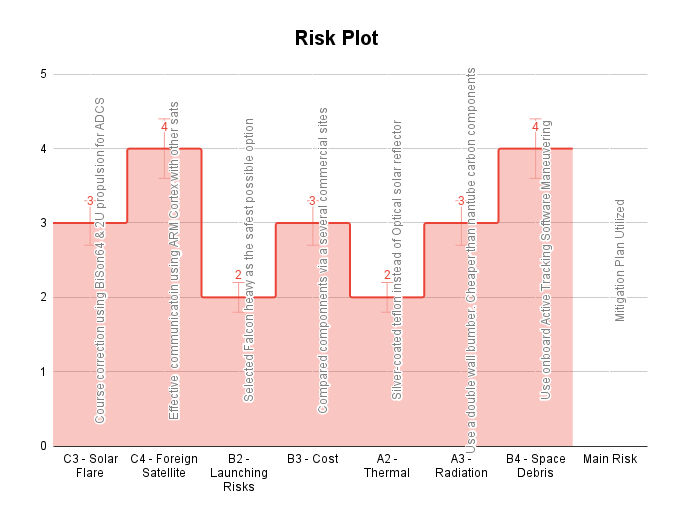
\includegraphics[width=\textwidth,frame, height=11cm]{Images/rplot.png}
    \caption{Risk Control}
    \label{fig:rplot}
\end{figure}

\subsection{Alternatives}
\begin{itemize}[noitemsep]
  \item 
Optical solar reflector to counter solar flares can be used  as cheaper alternatives instead of nanotube coating. 
  \item 
  Double wall bumpers were considered be used to further avoid thermal limitations. 
  \item 
  Alternate possible design considered as seen in Figure \ref{fig:alter}. Even if they can be used by switching up the axis of symmetry, there isn't enough area to put the solar cells on the side of frame. It can be possible considering lowering down the power budget for the cubesat.
\end{itemize}
\begin{figure}
    \centering
    \subfloat[Set up 1]{{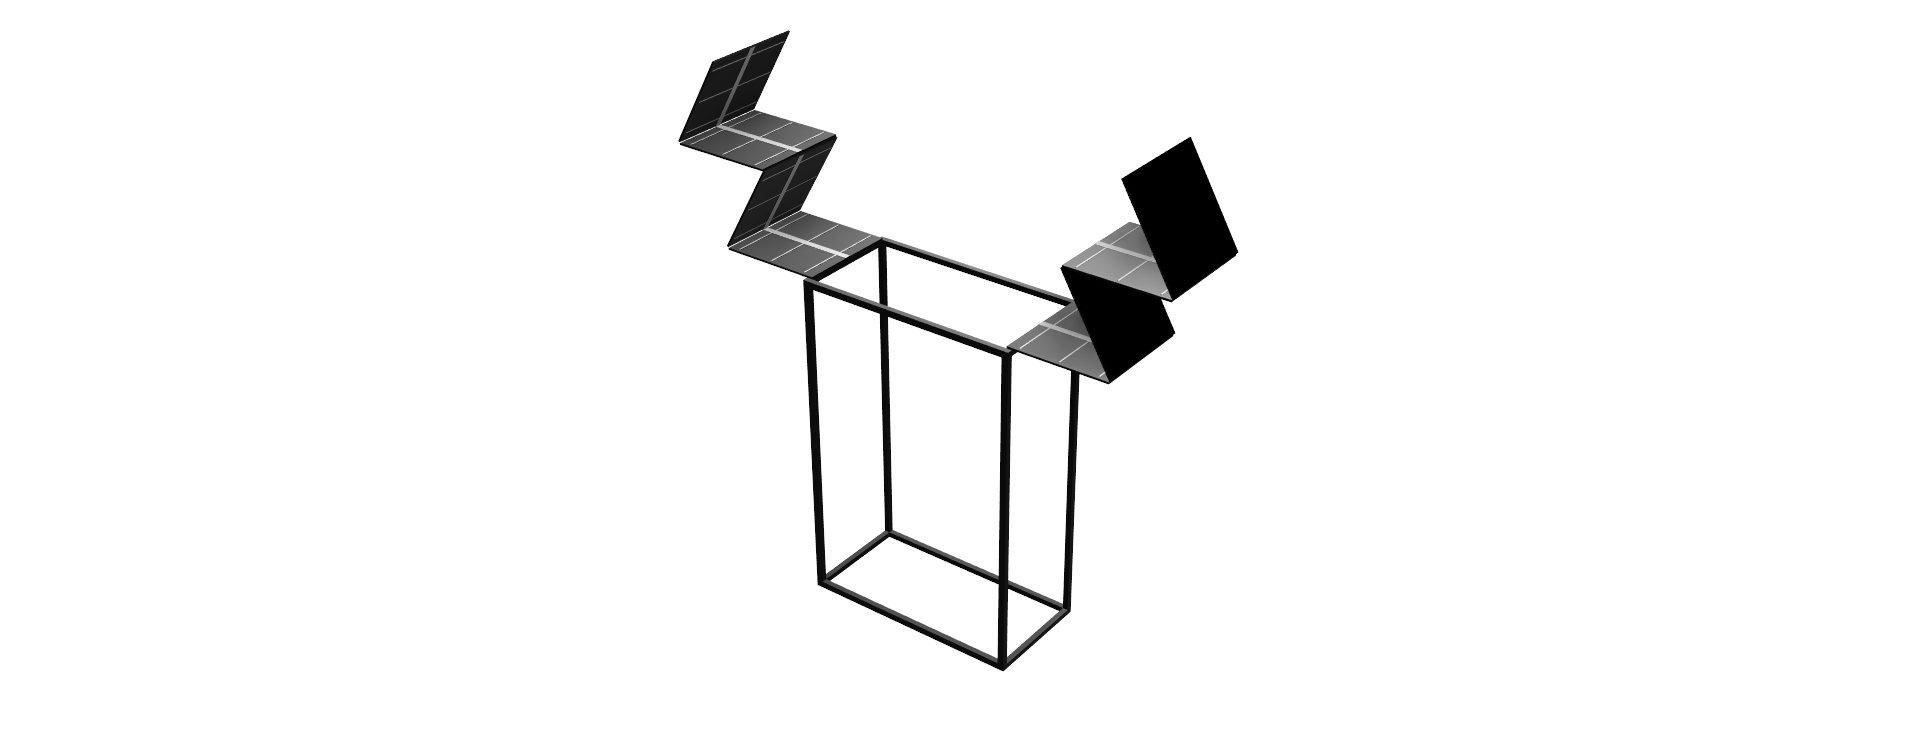
\includegraphics[width=8cm]{Images/a1.png} }}\label{fig:a1}
    \qquad
    \subfloat[Set up 2]{{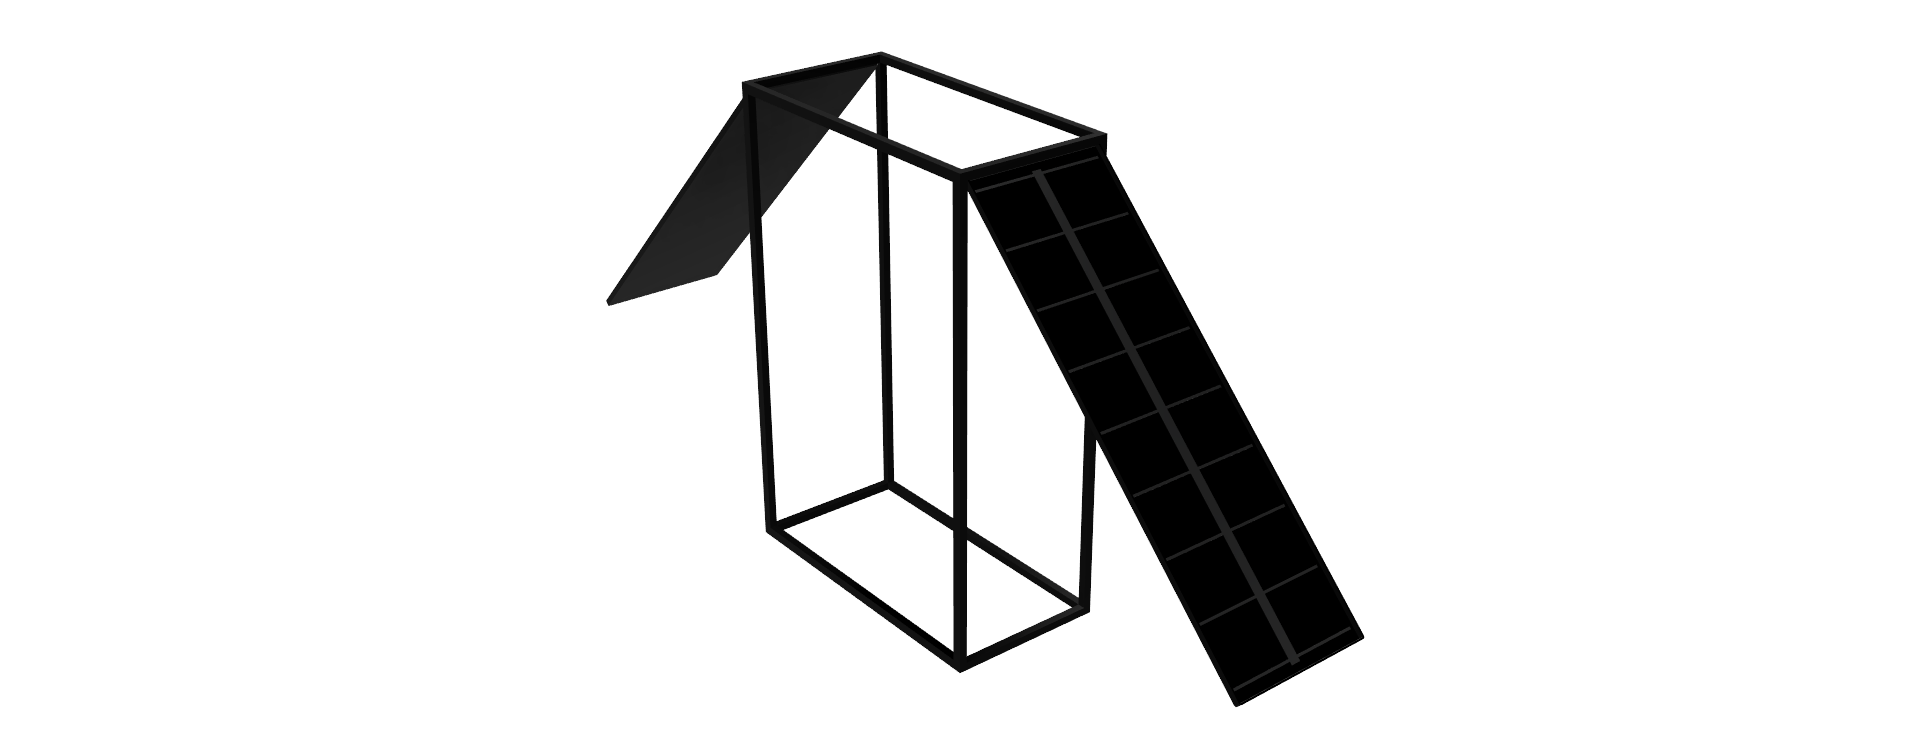
\includegraphics[width=8cm]{Images/a2.png} }}\label{fig:a2}
    \caption{Alternative frames considered}
    \label{fig:alter}
\end{figure}
\subsection{Technology Gaps and Trades}

Project HurriSat is designed by focusing on detailed component requirement and constraint in mind. Although goal is to aim for the safest and efficient spacecraft design possible, we are very limited on basis of cost and technological gap. The trade off is finding cheap yet good enough components, ride sharing for launch, and not nano-carbon framing and such. The list below highlights some of the challenges faced during this project.

\begin{itemize}[noitemsep]
  \item 
  Launching mechanisms can only be determined by NASA and SpaceX mechanics. 
  \item 
  The ADCS and OBC can be combined for a an advanced all in one components, had there been no halt in electronics production due to the pandemic. 
    \item 
    Actual stress, thermal and radiation  values may vary since we’re not manufacturing the cubesats. 
  \item 
  Prices are subject to change based on demand and supply
\end{itemize}
